% Original teaching architecture; reflow when labels or canvas change.
\documentclass[tikz,border=0pt]{standalone}
\def\FigureLanguage{en}
% Input after documentclass, before begin{document}; XeLaTeX/LuaLaTeX.
% Authors may define the Figure*Font commands before input to override defaults.
% English-only documents can set FigureLanguage=en without loading CJK support.
\providecommand{\FigureLanguage}{zh}
\providecommand{\FigurePrimary}{zh}
\makeatletter
\@ifundefined{ifFigureEnglishOnly}{%
  \newif\ifFigureEnglishOnly
  \def\FigureFontEnglishMode{en}%
  \edef\FigureFontSelectedMode{\FigureLanguage}%
  \ifx\FigureFontSelectedMode\FigureFontEnglishMode\FigureEnglishOnlytrue\fi
}{}
\makeatother
\providecommand{\FigureCJKFont}{SimSun}
\providecommand{\FigureLatinFont}{Times New Roman}
\providecommand{\FigureMathFont}{TeX Gyre Termes Math}
\ifFigureEnglishOnly
  \usepackage{fontspec}
  \typeout{FIGURE-CJK-FONT: not requested (English-only)}
\else
  \usepackage[UTF8,fontset=none]{ctex}
\fi
\usepackage{amsmath}
\usepackage{unicode-math}
\ifFigureEnglishOnly\else
\IfFontExistsTF{\FigureCJKFont}
  {\setCJKmainfont{\FigureCJKFont}\typeout{FIGURE-CJK-FONT: \FigureCJKFont}}
  {\setCJKmainfont{FandolSong-Regular}
   \typeout{FIGURE-CJK-FONT: FandolSong-Regular (fallback)}
   \PackageWarningNoLine{paperfigure}{Chinese font fallback: FandolSong-Regular}}
\fi
\IfFontExistsTF{\FigureLatinFont}
  {\setmainfont{\FigureLatinFont}\typeout{FIGURE-LATIN-FONT: \FigureLatinFont}}
  {\setmainfont{Latin Modern Roman}
   \typeout{FIGURE-LATIN-FONT: Latin Modern Roman (fallback)}
   \PackageWarningNoLine{paperfigure}{Latin font fallback: Latin Modern Roman}}
\IfFontExistsTF{\FigureMathFont}
  {\setmathfont{\FigureMathFont}\typeout{FIGURE-MATH-FONT: \FigureMathFont}}
  {\setmathfont{latinmodern-math.otf}
   \typeout{FIGURE-MATH-FONT: Latin Modern Math (fallback)}
   \PackageWarningNoLine{paperfigure}{Requested math font unavailable; using Latin Modern Math}}
% For individual bold letters/Greek symbols, not a replacement for bold equations.
% symbf follows bold-style; use symbfup/symbfit for explicit upright/italic.
\providecommand{\FigureBoldSymbol}[1]{\symbf{#1}}

\newcommand{\FigureLabel}[4][]{\parbox[c]{#1}{\centering #3\par}}
\usetikzlibrary{arrows.meta}
\begin{document}
\fontsize{9.5}{11.875}\selectfont
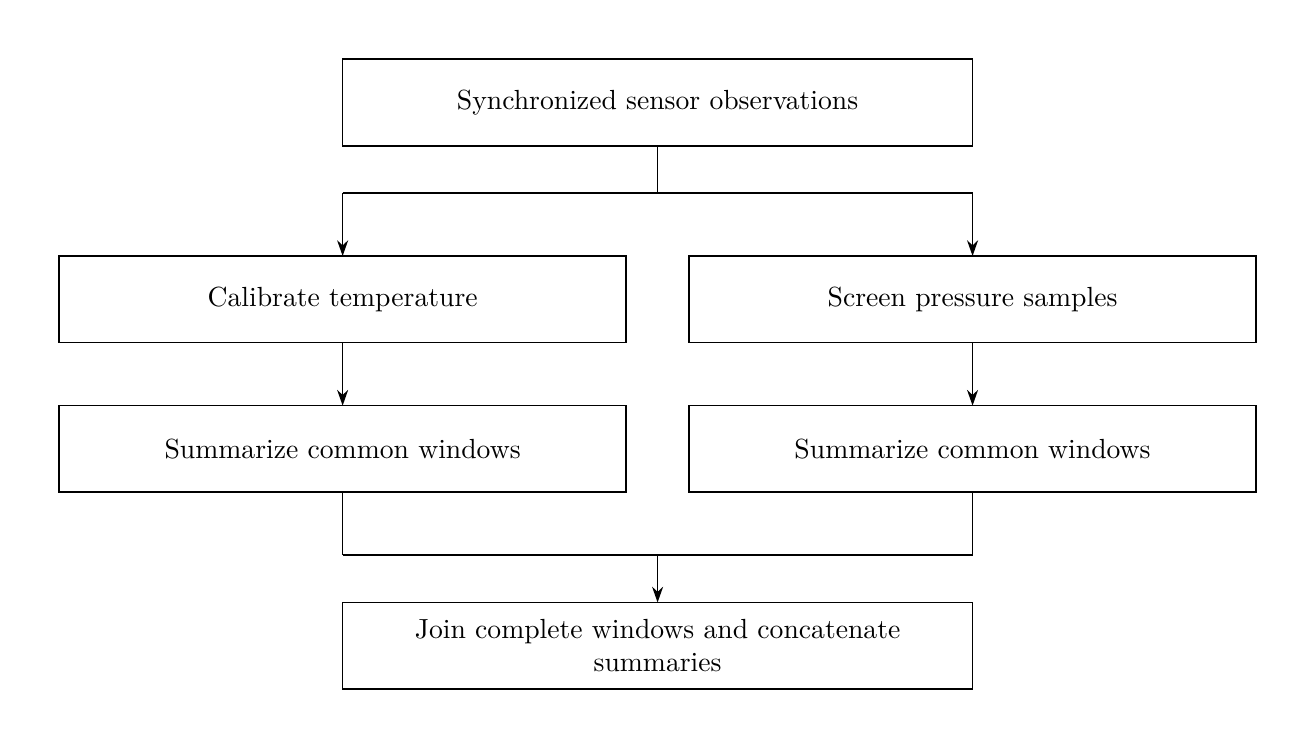
\begin{tikzpicture}[x=1mm,y=-1mm,line width=.6pt,
 every node/.style={inner sep=0pt,outer sep=0pt},>={Stealth[length=2mm,width=1.4mm]}]
\path[use as bounding box] (0,0) rectangle (160.000000,88.000000);
\draw (40.000000,4.000000) rectangle (120.000000,15.000000);
\draw (4.000000,29.000000) rectangle (76.000000,40.000000);
\draw (84.000000,29.000000) rectangle (156.000000,40.000000);
\draw (4.000000,48.000000) rectangle (76.000000,59.000000);
\draw (84.000000,48.000000) rectangle (156.000000,59.000000);
\draw (40.000000,73.000000) rectangle (120.000000,84.000000);
\draw (40.000000,21.000000) -- (80.000000,21.000000);
\draw (80.000000,21.000000) -- (120.000000,21.000000);
\draw (40.000000,67.000000) -- (80.000000,67.000000);
\draw (80.000000,67.000000) -- (120.000000,67.000000);
\draw (80.000000,15.000000) -- (80.000000,21.000000);
\draw[->] (80.000000,67.000000) -- (80.000000,73.000000);
\draw[->] (40.000000,21.000000) -- (40.000000,29.000000);
\draw[->] (40.000000,40.000000) -- (40.000000,48.000000);
\draw (40.000000,59.000000) -- (40.000000,67.000000);
\draw[->] (120.000000,21.000000) -- (120.000000,29.000000);
\draw[->] (120.000000,40.000000) -- (120.000000,48.000000);
\draw (120.000000,59.000000) -- (120.000000,67.000000);
\node[anchor=center] at (80.000000,9.500000) {\FigureLabel[76mm]{}{Synchronized sensor observations}{}};
\node[anchor=center] at (40.000000,34.500000) {\FigureLabel[68mm]{}{Calibrate temperature}{}};
\node[anchor=center] at (120.000000,34.500000) {\FigureLabel[68mm]{}{Screen pressure samples}{}};
\node[anchor=center] at (40.000000,53.500000) {\FigureLabel[68mm]{}{Summarize common windows}{}};
\node[anchor=center] at (120.000000,53.500000) {\FigureLabel[68mm]{}{Summarize common windows}{}};
\node[anchor=center] at (80.000000,78.500000) {\FigureLabel[76mm]{}{Join complete windows and concatenate summaries}{}};
\end{tikzpicture}
\end{document}
